% Bloque B: Aaron, 3:00. S5--S7. La solución: flujo, interfaz y
% arquitectura con piezas intercambiables.
\section{La solución}
\begin{frame}{ProductShot AI: una foto, cinco variaciones, una decisión por imagen}
  \centering% S5. Flujo de una sesión: de la foto al resumen, con rondas opcionales.
\begin{tikzpicture}[x=1cm,y=1cm]
  \path[use as bounding box] (0,-1.05) rectangle (13.5,0.75);
  \tikzset{paso/.style={box,font=\scriptsize,text width=2.1cm,minimum height=12mm}}
  \node[paso] (a) at (1.2,0) {\textbf{1. Foto}\\categoría y modo};
  \node[paso] (b) at (3.95,0) {\textbf{2. Controles}\\y segmentación};
  \node[acento,font=\scriptsize,text width=2.1cm,minimum height=12mm] (c) at (6.7,0) {\textbf{3. Generar}\\5 variaciones válidas};
  \node[bueno,font=\scriptsize,text width=2.1cm,minimum height=12mm] (d) at (9.45,0) {\textbf{4. Decidir}\\aceptar o rechazar\\cada una};
  \node[paso] (e) at (12.2,0) {\textbf{5. Resumen}\\verificado};
  \foreach \x/\y in {a/b,b/c,c/d,d/e} \draw[flow] (\x) -- (\y);
  \draw[flow,colAcento,dashed] (e.south) -- ++(0,-0.45) -| (c.south);
  \node[font=\scriptsize,text=colAcento,fill=white,inner sep=1pt] at (9.45,-0.82) {otra ronda que parte de las decisiones (máximo 3)};
\end{tikzpicture}

  \par\medskip
  {\small Cinco estilos por ronda: \textbf{estudio} $\cdot$ \textbf{natural} $\cdot$
  \textbf{cálido} $\cdot$ \textbf{lifestyle} $\cdot$ \textbf{minimalista}\par}
  \takeaway{La IA propone; la persona decide y el sistema registra cada decisión.}
  \source{Alcance: un solo producto pequeño, rígido y de preferencia opaco. No reconstruye caras ocultas ni la forma en 3D.}
  \note{Aaron. 3:00--4:00 (60 s). Así funciona. La persona sube una foto,
  elige la categoría y el modo. El sistema revisa la foto, separa el
  producto del fondo y genera exactamente cinco variaciones, una por
  estilo: estudio, natural, cálido, lifestyle y minimalista. La persona
  acepta o rechaza cada una, con un motivo opcional. Un agente redacta un
  resumen de esas decisiones y, si quiere, pide otra ronda de cinco que
  parte de lo que decidió; hasta tres rondas. El alcance es acotado: un
  producto pequeño, rígido y de preferencia opaco. No inventamos lados que
  la foto no muestra.}
\end{frame}

\begin{frame}{La interfaz: web móvil en cuatro pasos}
  \begin{columns}[c]
    \begin{column}{0.22\textwidth}
      \centering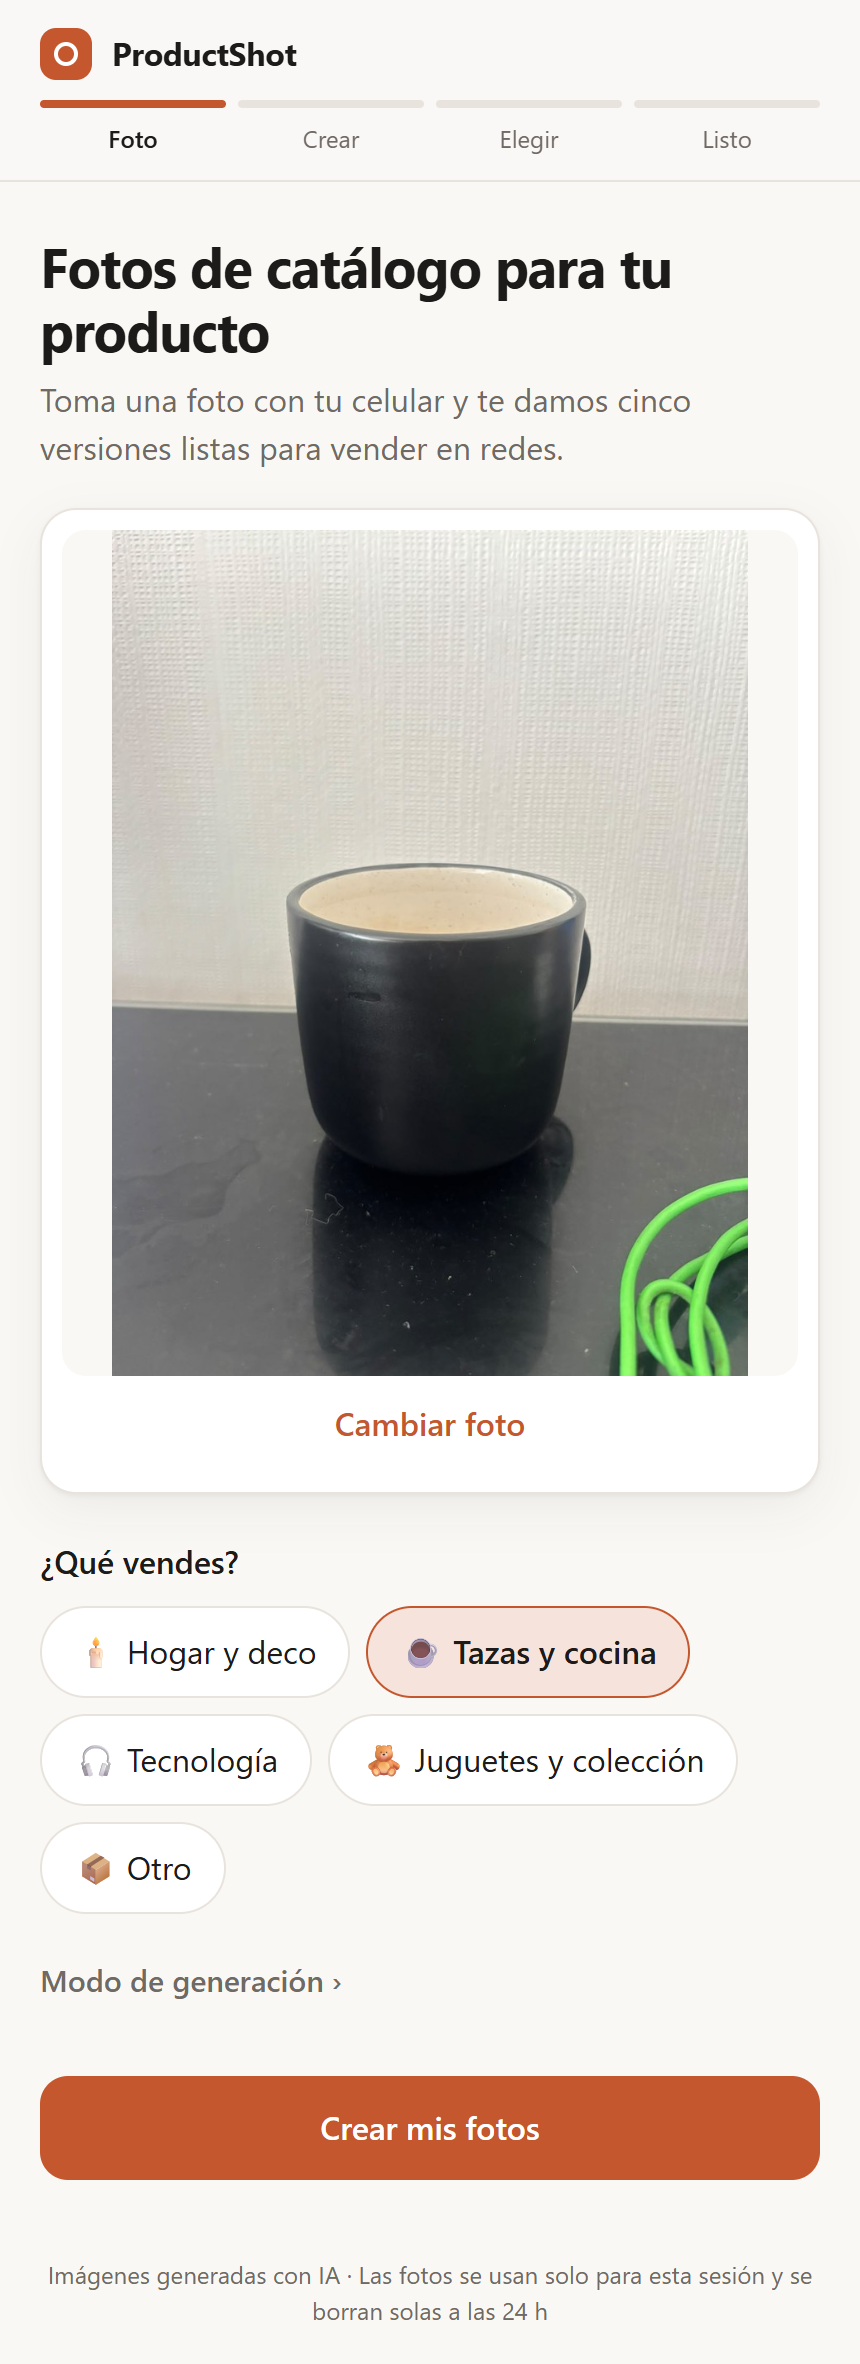
\includegraphics[height=5.6cm]{fig/ui_upload.png}
    \end{column}
    \begin{column}{0.42\textwidth}
      \centering
      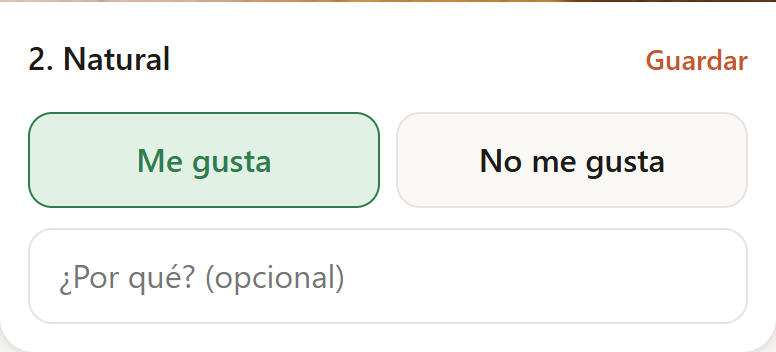
\includegraphics[width=0.9\linewidth]{fig/ui_decision_detail.png}\par\medskip
      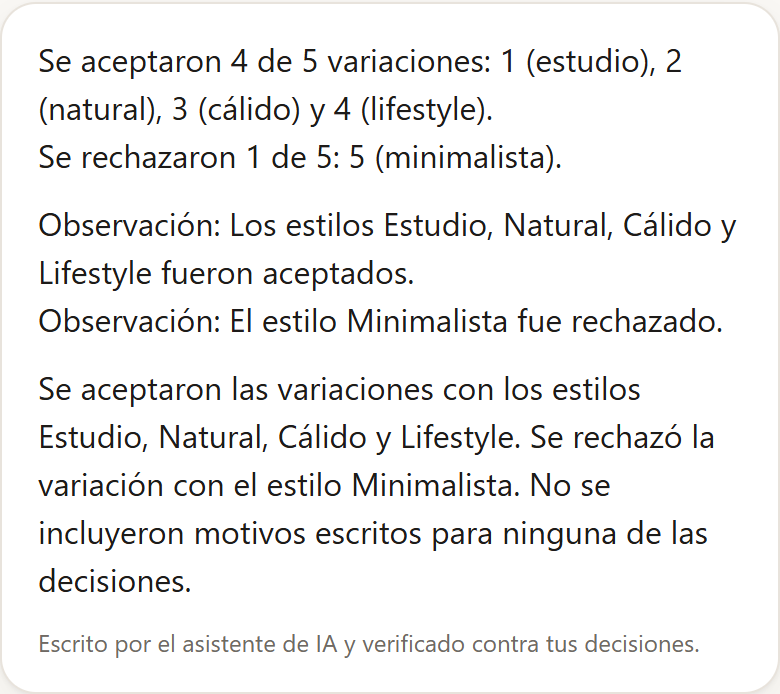
\includegraphics[height=3.0cm]{fig/ui_summary_detail.png}
    \end{column}
    \begin{column}{0.30\textwidth}\small
      \textbf{Foto} $\rightarrow$ \textbf{Crear} $\rightarrow$ \textbf{Elegir} $\rightarrow$ \textbf{Listo}\par\medskip
      Cámara o galería, en el celular.\par\medskip
      Aceptar o rechazar cada imagen, con un motivo opcional.\par\medskip
      Resumen y aviso del plazo de borrado.\par\medskip
      {\scriptsize También hay un panel en Gradio para ver y cambiar la máscara.}
    \end{column}
  \end{columns}
  \source{Capturas de la sesión de prueba con la taza.}
  \note{Aaron. 4:00--5:00 (60 s). La interfaz principal es una web pensada
  para el celular, con cuatro pantallas: Foto, Crear, Elegir y Listo. Se
  puede usar la cámara o la galería. En Elegir, cada imagen tiene dos
  botones, aceptar o rechazar, y un campo opcional para el motivo. Al
  final aparece el resumen y el aviso de cuándo se borran las fotos. Para
  el equipo también hay un panel en Gradio, que muestra la máscara y deja
  reemplazarla. Las dos interfaces hablan con la misma API.}
\end{frame}

\begin{frame}{Arquitectura: la API no necesita GPU}
  \centering% S7. Arquitectura: API sin GPU, workers en Modal y Gemini para el resumen.
\begin{tikzpicture}[x=1cm,y=1cm]
  \path[use as bounding box] (0,-0.35) rectangle (13.5,4.6);
  \tikzset{dflow/.style={flow,{Stealth[length=2mm]}-{Stealth[length=2mm]}}}
  \tikzset{pieza/.style={box,font=\scriptsize,text width=3.3cm,minimum height=11mm}}
  \node[pieza] (ui) at (6.75,4.0) {\textbf{Persona usuaria}\\web \texttt{/app} o Gradio \texttt{/ui}};
  \node[acento,font=\scriptsize,text width=3.6cm,minimum height=11mm] (api) at (6.75,2.25) {\textbf{FastAPI + sesiones}\\estados, validación, trabajos};
  \node[pieza] (db) at (1.95,2.25) {\textbf{SQLite + archivos}\\borrado a las 24\,h};
  \node[pieza] (llm) at (11.55,2.25) {\textbf{Gemini}\\solo decisiones y motivos};
  \node[box,font=\scriptsize,text width=4.2cm,minimum height=11mm,draw=colVenta,text=colVenta,fill=colVenta!8] (q) at (3.9,0.35) {\textbf{Worker intermedio} (Modal, H100)\\BiRefNet + Qwen-Image + controles};
  \node[box,font=\scriptsize,text width=4.2cm,minimum height=11mm,draw=colCompra,text=colCompra,fill=colCompra!8] (s) at (9.6,0.35) {\textbf{Worker avanzado} (Modal, L4)\\SDXL inpainting + LoRA};
  \draw[dflow] (ui) -- node[right,font=\scriptsize]{HTTP} (api);
  \draw[dflow] (api) -- (db);
  \draw[dflow] (api) -- (llm);
  \draw[dflow] (api) -- (q);
  \draw[dflow] (api) -- (s);
\end{tikzpicture}

  \takeaway{Puertos y adaptadores: el mismo código corre simulado o con los modelos reales.}
  \note{Aaron. 5:00--6:00 (60 s). Arriba, la persona usa la web o Gradio,
  que llaman por HTTP a una API en FastAPI. El servicio de sesiones
  controla los estados y guarda todo en SQLite y una carpeta de imágenes.
  Los modelos pesados no corren en la API: están en dos workers de Modal,
  el intermedio en H100 y el avanzado en L4, y el resumen lo escribe
  Gemini. Cada pieza es un adaptador que se elige por configuración. Por
  eso el mismo código corre en modo simulado, sin GPU ni red, que usamos
  para desarrollar y para las pruebas, o en modo real. El costo: más
  contratos entre procesos y dependencia de la red. Isaac explica los
  modelos.}
\end{frame}
